\graphicspath{{img/ch2}}


\section{Lunar Pit Geological Characteristics}

\subsection{Morphological Characteristics}

Lunar pits exhibit distinct morphological features that provide critical insights into their geological origins and evolution. Typically characterized by funnel-shaped upper regions leading into near-vertical walls, these pits often terminate in flat or slightly concave floors \cite{new-wagner, lunar-pits-numerical-modelling, lunar-pit-distribution}. The sharp transition between the sloping entrance and vertical walls suggests that these features form primarily due to sudden roof collapses above subsurface voids, rather than gradual erosion processes \cite{lunar-pits-numerical-modelling, new-wagner}.

\begin{figure}[h!]
    \centering
    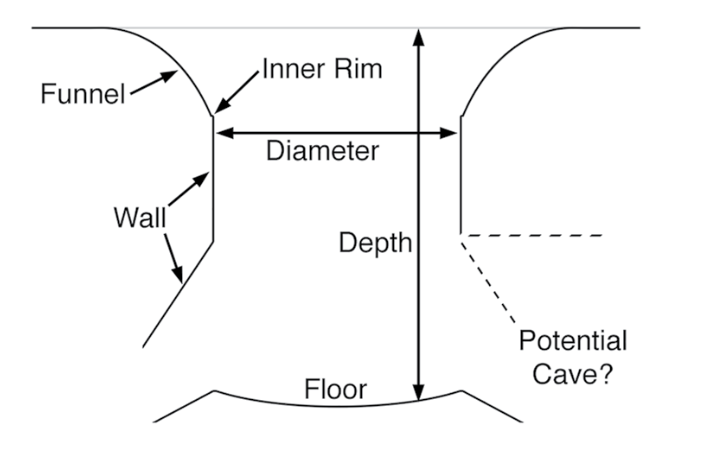
\includegraphics[width=0.5\linewidth]{lunar_pit_schema.png}
    \caption{A simplified schematic of a generic lunar pit cross-section showing key morphological features (adapted from \cite{new-wagner}).}
    \label{fig:lunar-pit-schema}
\end{figure}

High-resolution images from the Lunar Reconnaissance Orbiter (LRO) Narrow Angle Camera (NAC) have revealed significant details, such as stratified layering within pit walls, which likely correspond to successive volcanic flow events. These layers provide critical geological records of ancient lunar volcanism \cite{lunar-pits-entrances-to-caves, Carrer2024}. Overhangs within pits, such as those in Mare Tranquillitatis and Marius Hills, indicate access to extensive subsurface voids consistent with collapsed lava tubes. These voids could extend tens of meters and present exciting opportunities for future robotic exploration missions \cite{lunar-pits-numerical-modelling, radar-observations-lava-tubes}.

The bases of lunar pits commonly accumulate boulders and regolith, which can obscure deeper portions of the pits and affect depth measurements. Concave floors can alter the perceived depth by visually increasing the vertical extent of the pit's interior relative to its surroundings \cite{lunar-pit-distribution, new-wagner}. This contrasts with traditional impact craters, which are characterized by raised rims and ejecta blankets.

Over geological timescales, lunar pits degrade due to micrometeoroid impacts, thermal cycling, and seismic activity. These processes erode walls and rims, depositing debris at the base. Mare Tranquillitatis, which retains sharp walls and minimal infill, contrasts with Marius Hills pits, where smoother, partially infilled floors indicate older, more degraded structures. This variation in preservation demonstrates the gradual evolution of lunar pits over hundreds of millions of years, largely independent of surrounding terrain age \cite{lunar-pit-distribution, radar-observations-lava-tubes, newer-thermal}.

\begin{figure}[H]
    \centering
    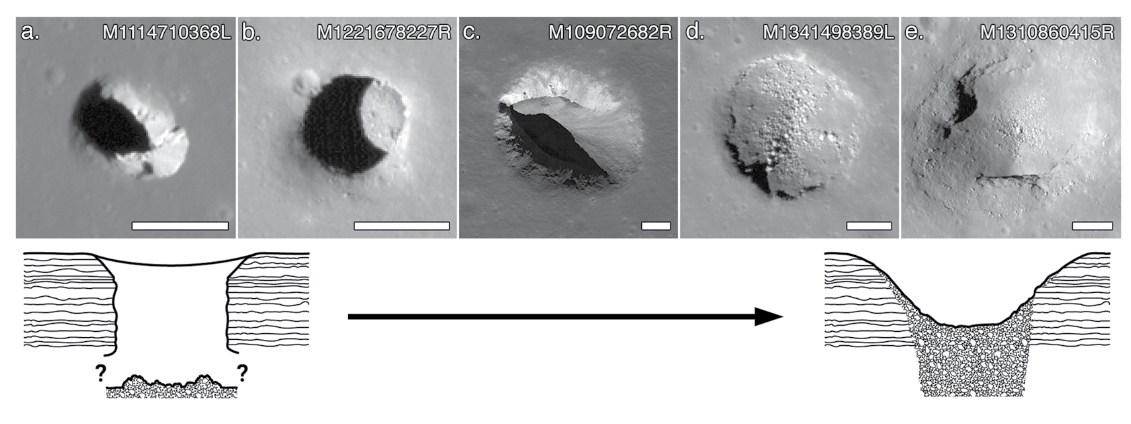
\includegraphics[width=0.85\linewidth]{closed_and_open_cavities.png}
    \caption{Progression of lunar pit degradation, illustrating gradual erosion and regolith deposition over time. The figure shows different lunar pits in various stages of erosion (adapted from \cite{new-wagner}).}
    \label{fig:lunar-pit-degradation}
\end{figure}

\subsection{Geographical Distribution and Formation Mechanisms}

Lunar pits are distributed across three primary geological settings: mare basalts, impact melt deposits, and highland terrain. Each setting reflects distinct formation mechanisms and geological implications \cite{lunar-pit-distribution, radar-observations-lava-tubes}.

\begin{figure}[H]
    \centering
    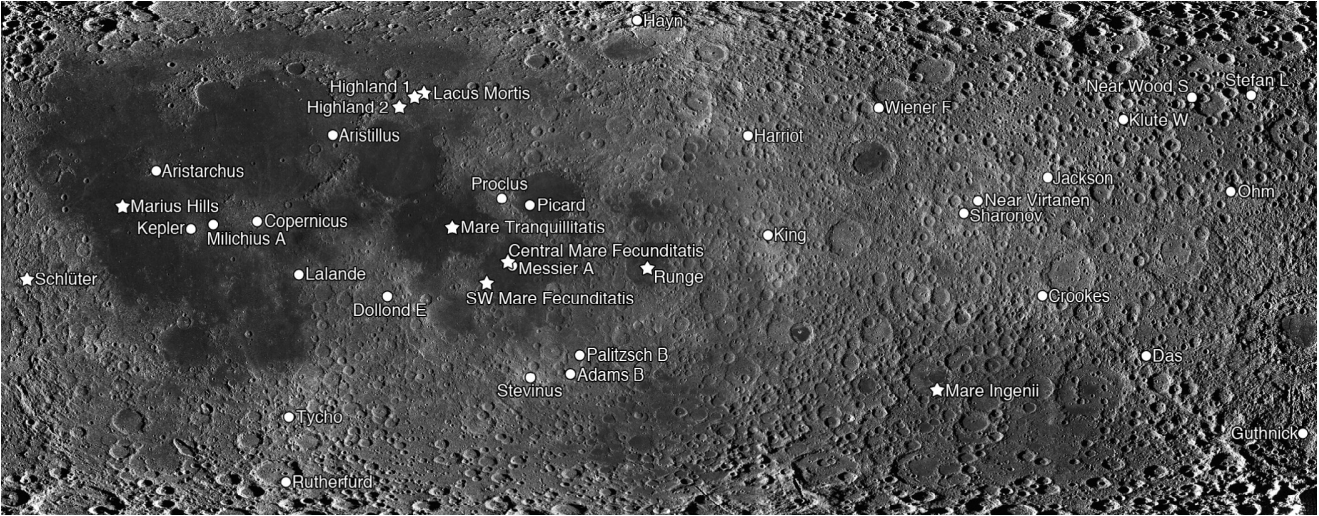
\includegraphics[width=0.98\linewidth]{map-lunar-pits-rough.png}
    \caption{Map of lunar pits: eight in mare basalts, two in highlands (stars), and 29 in impact melt deposits (dots). Figure adapted from \cite{lunar-pit-distribution}. This map is from 2014, currently, more then 300 lunar pits were discovered.}
    \label{fig:map-lunar-pits}
\end{figure}

\paragraph{Mare Basalts}
Pits in mare regions, such as Marius Hills and Mare Tranquillitatis, are predominantly linked to volcanic activity. These pits are hypothesized to form through the collapse of lava tube roofs, as overlying material becomes unstable and collapses into voids below \cite{lunar-pits-entrances-to-caves, radar-observations-lava-tubes}. Radar and imaging data from Mare Tranquillitatis reveal extensive subsurface voids consistent with intact lava tubes, which serve as potential habitats or scientific exploration targets \cite{Carrer2024, radar-observations-lava-tubes}.

\begin{figure}[H]
    \centering
    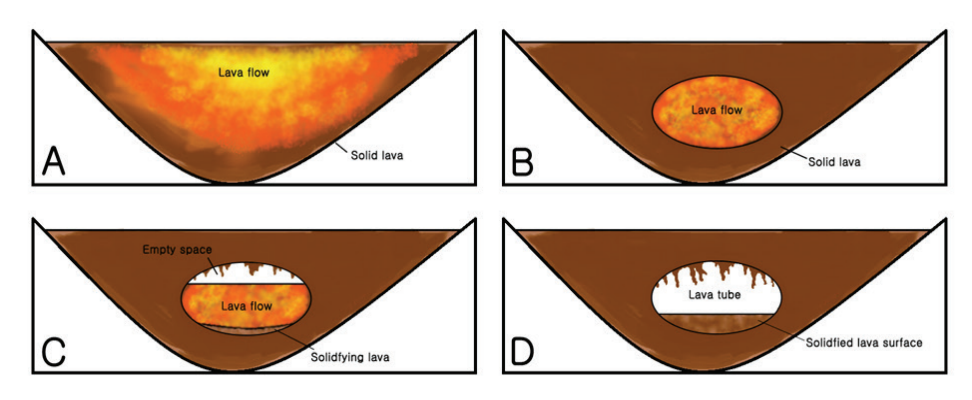
\includegraphics[width=0.7\linewidth]{lava_tube_formation_schema.png}
    \caption{Stages of lunar lava tube formation, illustrating crust solidification, lava drainage, and resulting voids (adapted from \cite{lunar-pits-entrances-to-caves}).}
    \label{fig:lava-tube-formation-schema}
\end{figure}

\paragraph{Impact Melt Deposits}
Pits found within impact craters, such as Tycho and Copernicus, form due to high-energy impacts that fracture and compress the lunar crust, generating molten material. As this molten material cools, thermal contraction creates cracks and fractures that eventually collapse into pits. These features are typically circular in shape, lack overhangs, and have no association with lava flows \cite{clrn-impact-melt, lunar-pits-numerical-modelling}.

\begin{figure}[H]
    \centering
    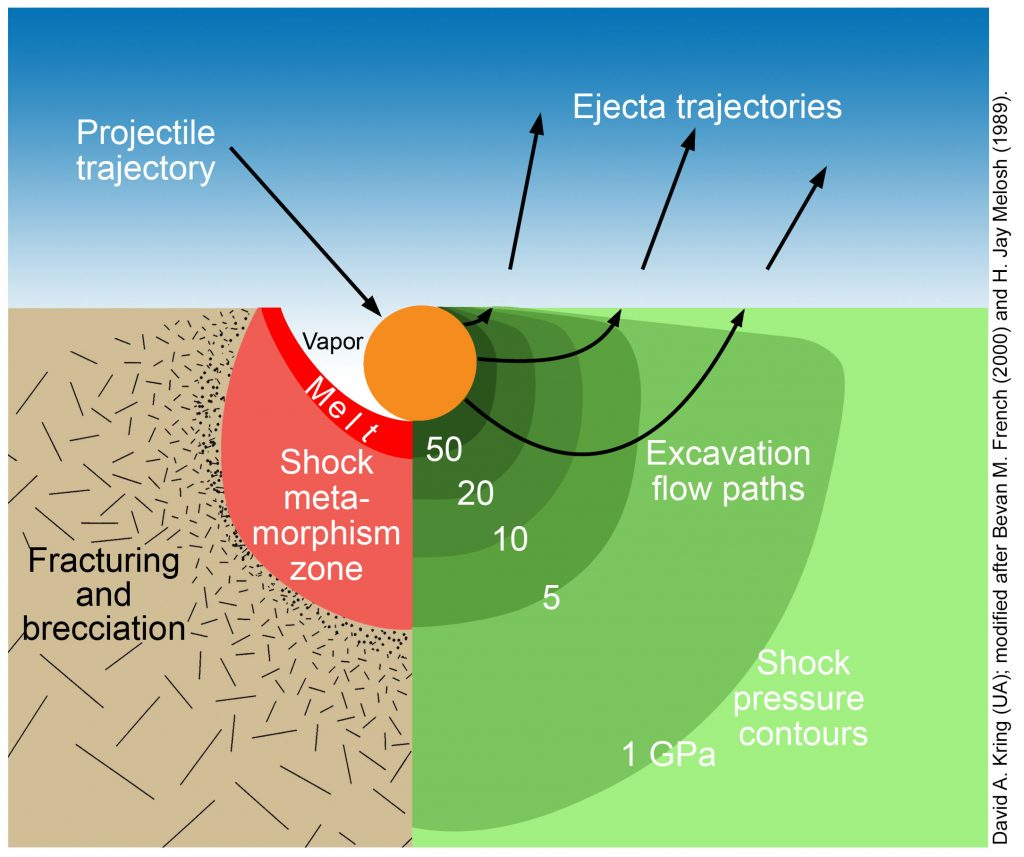
\includegraphics[width=0.42\linewidth]{Impact-Shock-Pressures-and-Their-Effects-1024x857.jpg}
    \caption{Impact dynamics illustrating pressure zones, molten material, and the formation of cracks contributing to pit formation in impact melt deposits (adapted from \cite{clrn-impact-melt}).}
    \label{fig:impact-melt}
\end{figure}

\paragraph{Highland Terrain}
Highland pits, such as those in Lacus Mortis, are thought to result from tectonic stresses and extensional faulting. These pits typically form near graben systems or faulted regions, where crustal stress generates fractures. Over time, localized collapses along these fault zones create pits with sharp, near-vertical walls. Unlike mare pits, highland pits lack volcanic associations, emphasizing their tectonic origin \cite{new-wagner, lunar-pit-distribution}. 

While mare pits are often associated with extensive sublunarean cavities, highland pits generally lack direct evidence of such voids. Their formation mechanisms, primarily driven by tectonic activity, may result in smaller or less interconnected voids compared to those formed by lava tube collapses. Current studies, such as those by Wagner et al. (2022), have not confirmed large, accessible sublunarean cavities within highland terrain pits, limiting their potential for exploration of extensive underground structures \cite{lunar-pit-distribution, radar-observations-lava-tubes, cavities-selene-lavatubes}.

\begin{figure}[H]
    \centering
    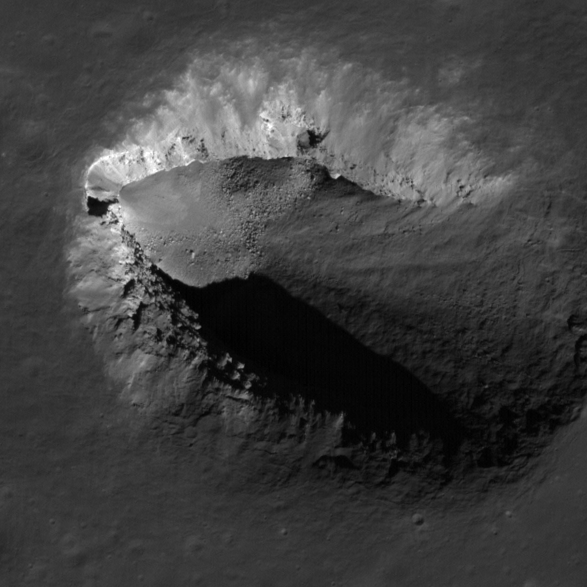
\includegraphics[width=0.33\linewidth]{lunar-pit-highland.png}
    \caption{Lunar Reconnaissance Orbiter Camera footage of Lacus Mortis Pit. Image adapted from: \url{https://www.lroc.asu.edu/atlases/pits}.}
    \label{fig:highland-lunar-pit}
\end{figure}

\paragraph{Impact-Induced Skylights}
Unlike the formation mechanisms described above, impact-induced skylights are not a primary formation mechanism but occur when small meteoroid impacts destabilize thin crusts overlying intact voids, such as lava tubes. Numerical simulations suggest that impacts create localized collapses, such as the 26-meter-thick roof collapse in Marius Hills, forming a skylight approximately 40 meters wide. These simulations highlight skylights as secondary features of great interest for exploration \cite{clrn-impact-melt, lunar-pits-numerical-modelling}.

\begin{figure}[H]
    \centering
    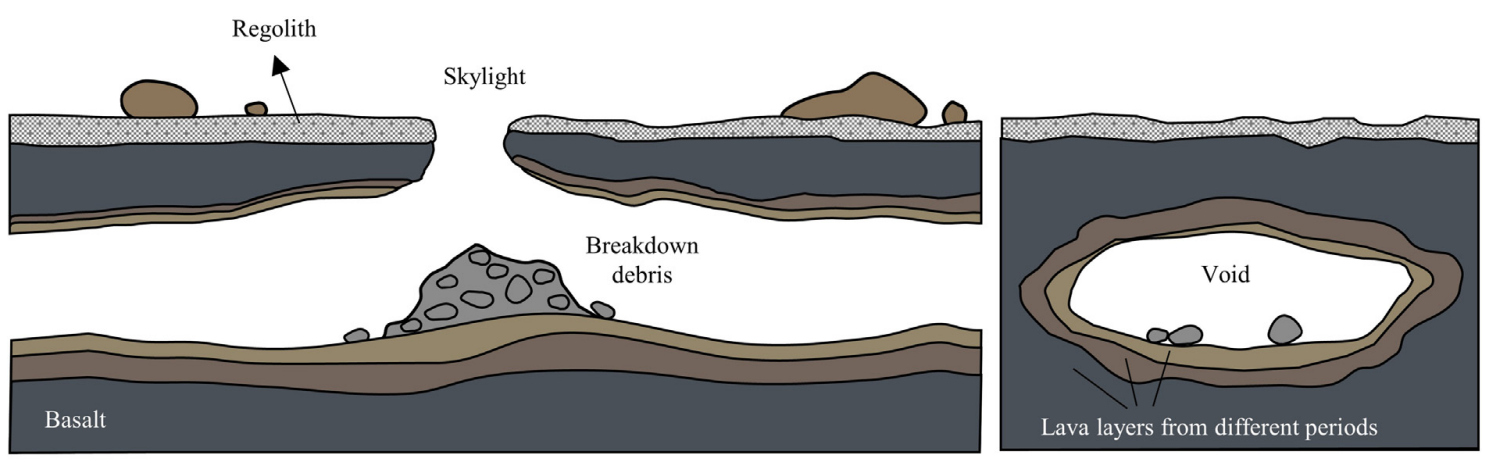
\includegraphics[width=0.99\linewidth]{lunar-pit-in-lava-tube.png}
    \caption{Cross section of a lunar tube with collapsed skylight (adapted from \cite{bases-feng}).}
    \label{fig:impact-induced-skylight}
\end{figure}


\section{Earth Analog Structures for Lunar Studies}

Lava tubes and pits on Earth serve as valuable analogs for understanding similar structures on the Moon. These terrestrial features provide key insights into formation mechanisms, stability, and potential for scientific research and exploration.

\subsection{Earth Analog Structures for Lunar Studies}

Lava tubes on Earth, such as those in Hawaii, Iceland, and the Canary Islands, provide accessible models for studying the structural dynamics of their lunar counterparts. These tubes are formed by flowing lava that cools on the surface while the molten interior continues to flow, eventually draining to leave behind hollow tunnels. Detailed studies of these tubes reveal various morphologies, from smooth-walled passages to intricate branching systems, which mirror the complexity observed in lunar lava tubes \cite{bases-feng, sublunear-lava}.

\begin{figure}[H]
    \centering
    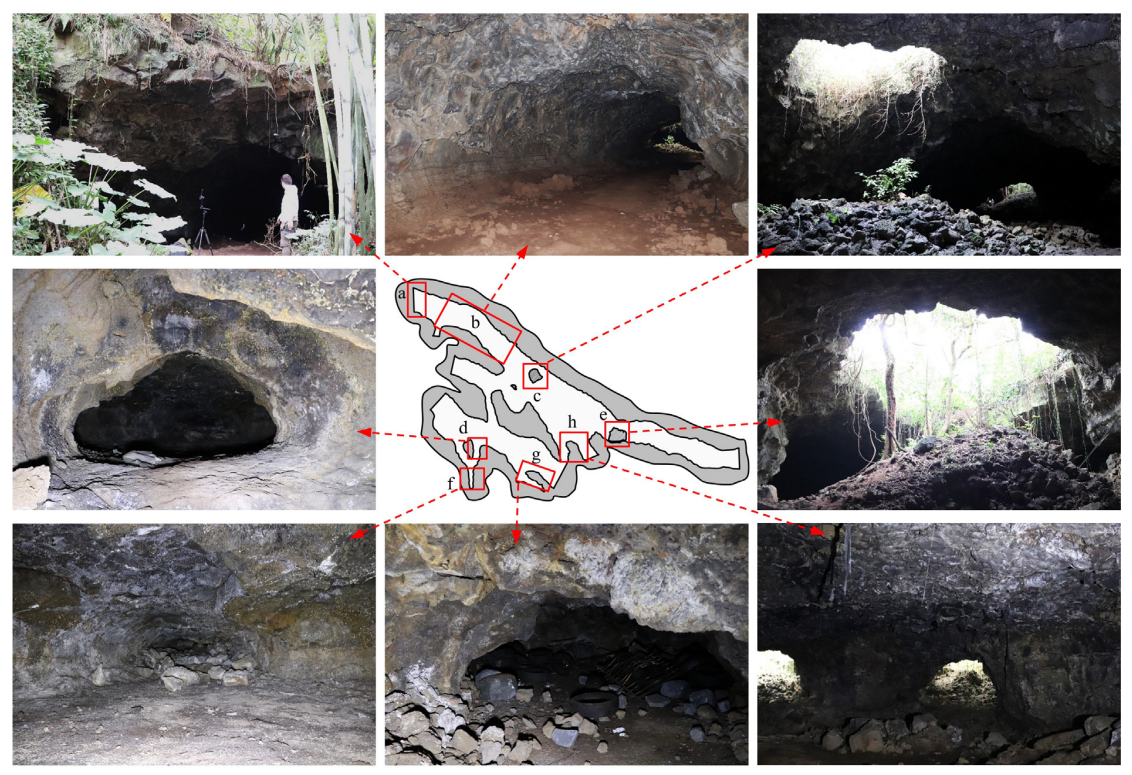
\includegraphics[width=0.8\linewidth]{earth-based-lavatube.png}
    \caption{A simplified map of the \textit{Seventy-Two Caves} terrestrial lava tube with photos from various parts of the cave system (adapted from \cite{bases-feng}).}
    \label{fig:terrestrial-lava-tubes}
\end{figure}

\subsection{Comparative Studies: Earth and Moon}

Pits and skylights on Earth, such as those found in Idaho, Victoria (Australia), and the Northern Borders of Saudi Arabia, share visual and structural similarities with lunar pits like those in the Stevinus, King, and Aristarchus regions. These features provide natural windows into subsurface voids and serve as critical sites for geological and environmental studies \cite{lunar-pits-entrances-to-caves, radar-observations-lava-tubes}. The comparative sizes and formation mechanisms offer unique perspectives on how gravitational differences and environmental conditions shape these features \cite{lunar-pit-distribution, bases-feng}.

\begin{figure}[H]
    \centering
    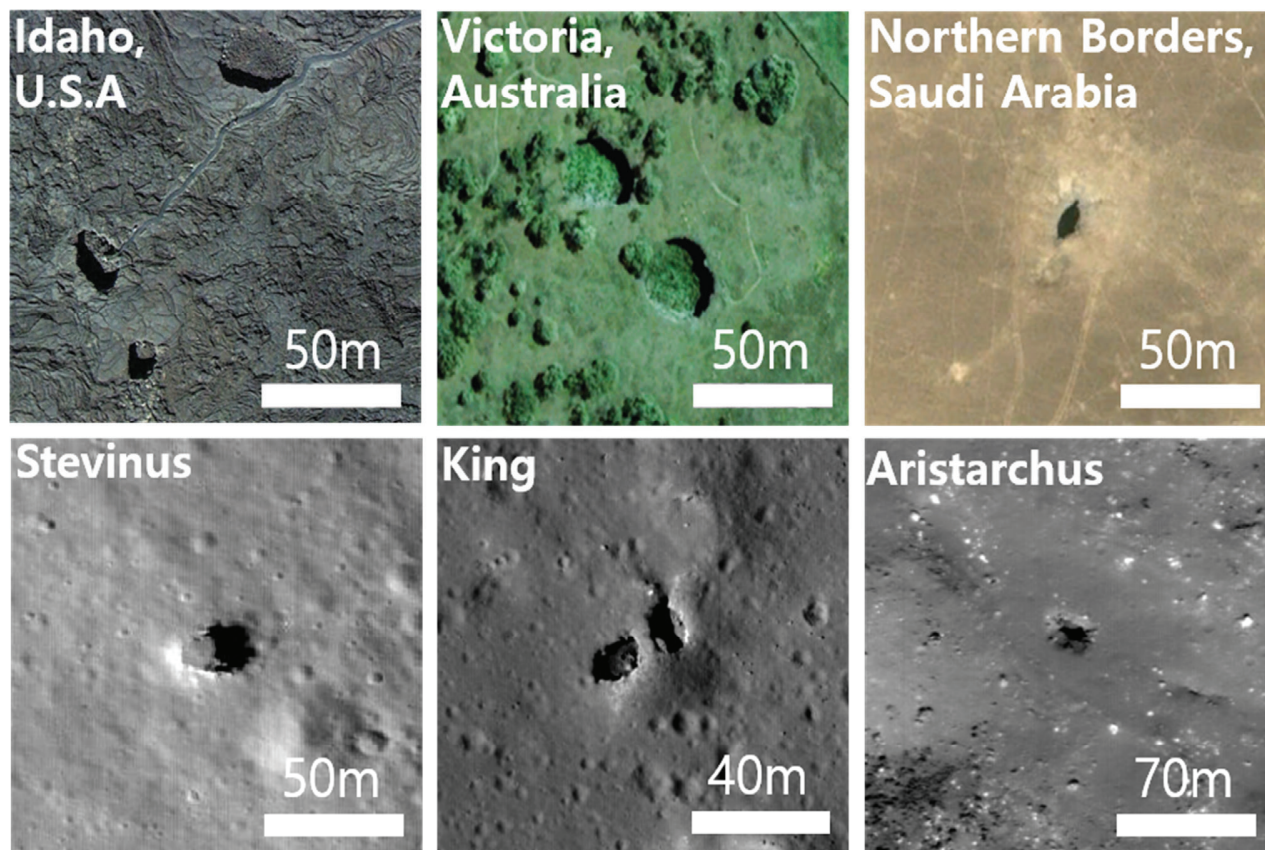
\includegraphics[width=0.8\linewidth]{terrestrial-vs-lunar-pits.png}
    \caption{Comparison of pits on Earth (top row) and the Moon (bottom row). Scale bars indicate relative sizes (adapted from \cite{lunar-pits-entrances-to-caves}).}
    \label{fig:earth-moon-pits}
\end{figure}

\subsection{Scientific Implications}

Studying terrestrial analogs provides critical insights for lunar exploration:
\begin{itemize}
    \item \textbf{Formation Mechanisms:} Understanding how terrestrial pits and lava tubes form informs theories about lunar geological processes \cite{sublunear-lava, radar-observations-lava-tubes}.
    \item \textbf{Structural Stability:} Investigating the long-term stability of terrestrial lava tubes aids in assessing the feasibility of using lunar lava tubes for habitation or scientific research \cite{bases-feng}.
    \item \textbf{Access and Exploration Techniques:} Testing rovers, mapping tools, and navigation systems in terrestrial lava tubes offers a controlled environment to refine techniques before deployment on the Moon \cite{kerber2023, esa-daedalus}.
\end{itemize}